\subsection{X線回折パターン}
図\ref{fig:fig6}に,メソMD計算で得たモデル1とモデル2の組織構造
に対するX線回折パターンを示す.グラフの横軸はX線の回折角$2\theta$[deg]を,
縦軸はX線強度$I$を表し,各々のグラフには,7つの異なる圧縮段階における
XRDパターンが示されている.また,図中に示した数値は,それら7つの段階
における乾燥密度と間隙率を表している.
ここには,圧縮の進行すなわち乾燥密度の増加に伴い,次第に強い回折ピークが
$2\theta=$6度付近に現れる様子が見られる.このピーク角度は,二層膨潤状態
にある粘土の層間距離に対応し,実験でも観測されるものである.
一方,回折ピークの鋭さは,組織構造が有する周期性を反映したものであり,
鋭いピークであるほど積層数が多いことを意味する.
この点においてモデル1とモデル2の回折パターンを比較すると,モデル2のピークは
モデル1に比べてやや鋭く,積層構造がより発達していることが分かる.
また,モデル1とモデル2の結果とも,乾燥密度が小さく,粘土分子が非常に緩く
堆積した状態でも,$2\theta=$5度付近にピークが見られる.このことは,
XRDパターンとして見た場合にも,圧縮の早い段階で積層構造が形成さること,
圧縮の進行により平均的な層間距離が次第に詰まってはくるものの,積層数自体は
あまり大きくならないことを示している.
%--------------------
\begin{figure}[h]
	\begin{center}
	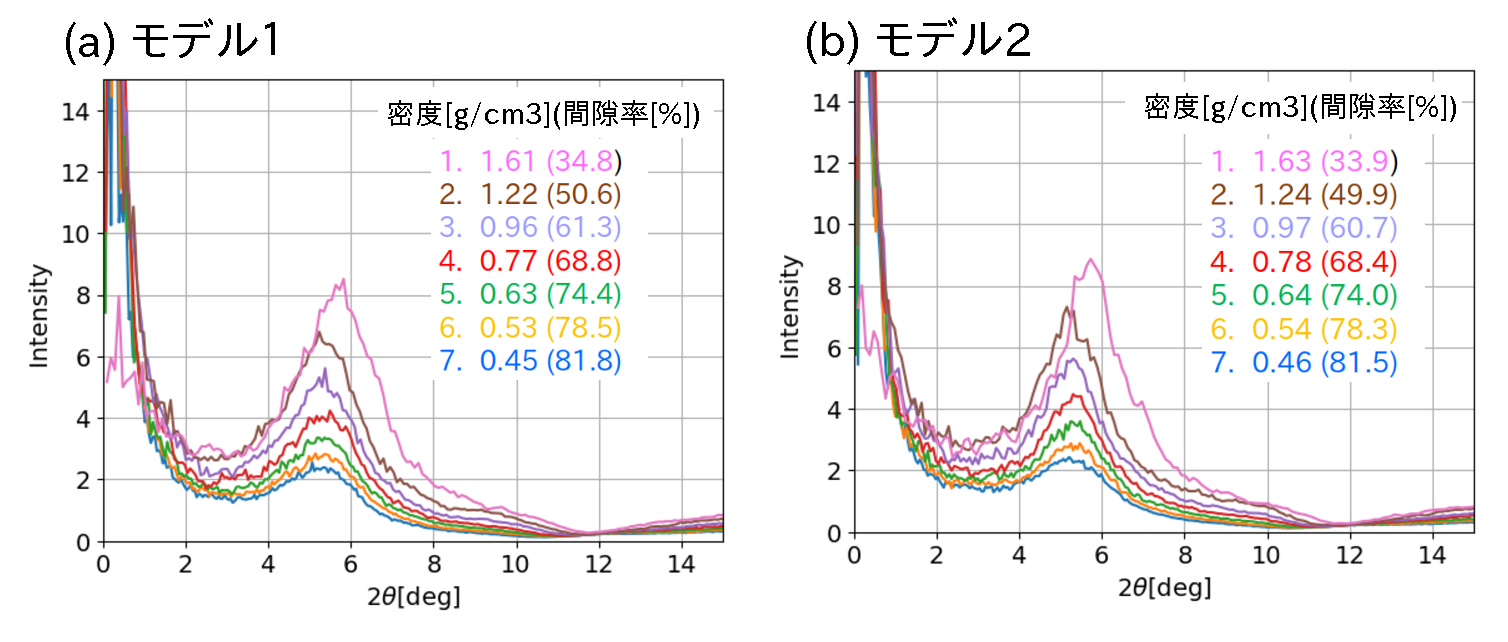
\includegraphics[width=1.0\linewidth]{Figs/fig6.eps} 
	\end{center}
	\caption{
		メソMDシミュレーションの結果から求めたX線回折パターン.
	} 
	\label{fig:fig6}
\end{figure}
%--------------------
\subsection{動径分布関数}
動径分布関数(RDF)の計算結果を図\ref{fig:fig7}に示す.XRDパターンと同様,ここでも,
モデル1および2に対する結果それぞれについて,7つの異なる密度において評価した
RDFをプロットしている.RDFのピークは,横軸で示された動径距離$r$で,
相対的に多数の粗視化粒子が存在することを表すものである.ここに示した結果では,
全てのケースでRDFは複数のピークを有しており,ピーク位置にあたる動径距離は
概ね1.5nm間隔で現れている.これは,二層膨潤状態における粘土層間距離に一致し,
平均的に二層膨潤状態にあること,また,組織構造中に見出される粘土分子の積層状態
が式(\ref{eqn:RDFn})のRDFで適切に評価されていることを示している.
ここで,乾燥密度によるRDFの変化に着目すると,RDFの値は乾燥密度の減少に応じて
増加傾向を示す一方,グラフの形状自体は大きく変化しないことが分かる.
これは,圧縮初期の段階で形成された積層構造が維持され,その後大きく発達することがない
ことを意味する.一方,モデル1とモデル2の結果の比較では,
モデル1で明確なピークが3つであるのに対し,モデル2では5つ程度のピークが
見られることが分かる.これは,モデル1と2の組織構造の示す平均的な積層数がそれぞれ
4層と6層であることを意味し,実験で得られるX線回折ピークの半値幅から推定される
結果に近い値となっている.これら,積層数と積層構造の形成時期に関する傾向は
XRDパターンから読み取ることができる傾向と整合している.
RDFとXRDパターンは,理論的には相互に変換可能である.そのため,両者の解釈はそもそも
一致すべきものである.ただし,本研究ではXRDパターンとRDFは異なる仮定の元,別の
方法で評価したものであることから,両者の結果から読み取れる情報が整合的であることは,
これら2つの分布関数の評価方法が妥当であることを裏付ける結果と言える.
%--------------------
\begin{figure}[h]
	\begin{center}
	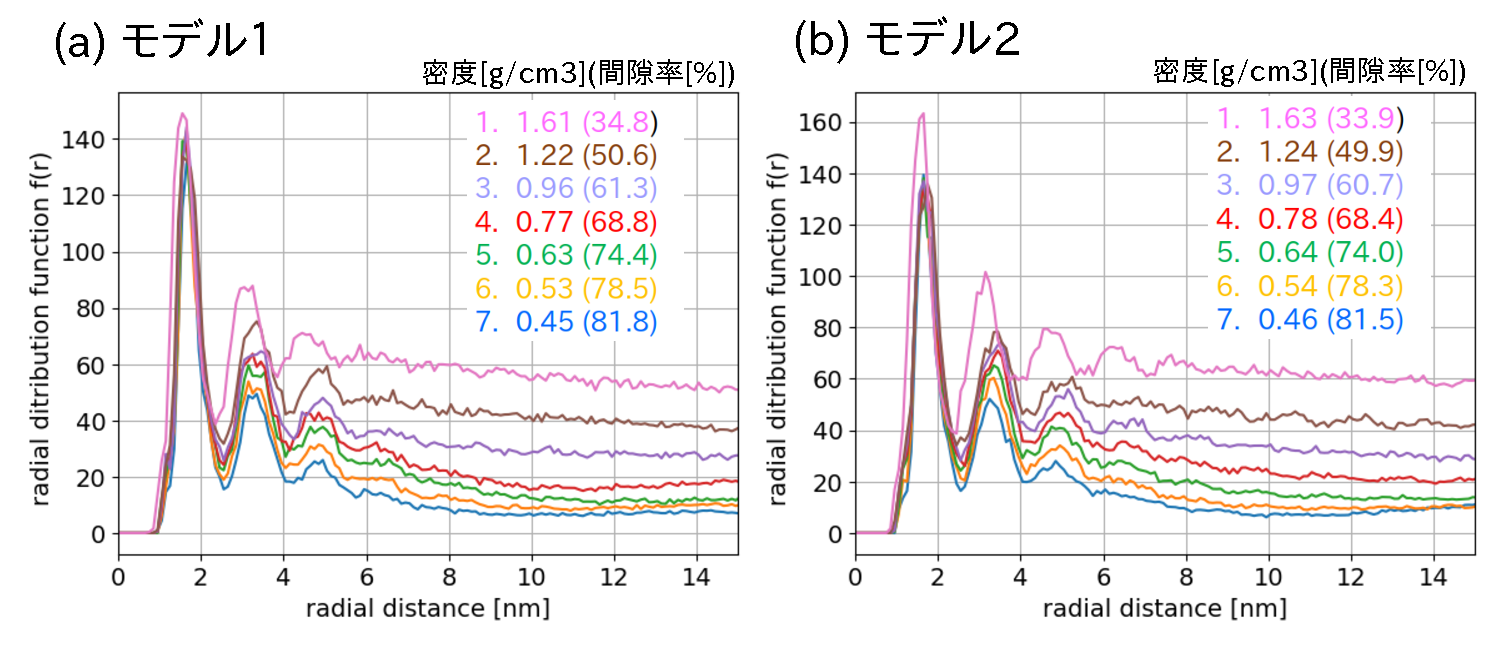
\includegraphics[width=1.0\linewidth]{Figs/fig7.eps} 
	\end{center}
	\caption{
		メソMDシミュレーションの結果から求めた動径分布関数.
	} 
	\label{fig:fig7}
\end{figure}
%--------------------
\subsection{数密度}
\subsubsection{確率密度関数}
局所密度を与える式(\ref{eqn:rhox_gen})において,$m_i=1$と置けば,
$\rho(\fat{x})$の値は粗視化粒子の数密度と一致する.
図\ref{fig:fig8}は,このことを利用して粒子の数密度を求めたもので,
数密度のヒストグラムを正規化して確率密度分布と見ることができる形で
示してある.ここでも,モデル1と2,それぞれ7つの異なる乾燥密度に
に対する結果が示されている.乾燥密度が低いとき,局所密度はゼロ付近で
大きな確率をとっている.これは,粘土層外の空隙が,ユニットセル内で広い
範囲を占めることを反映したもので,乾燥密度の増加に伴って低下を続け,
最終的には消失する.それと入れ替わるように,数密度0.6付近のピークが顕著
になる.ただし,密度0.6付近の緩やかなピークは,圧縮過程の初期段階から存在し,
これは,早い段階で粘土分子が凝集することを反映したものである.
なお,モデル1と2の結果を比較するとモデル2のピークがより鋭い.
これは,モデル2はモデル1に対して粒径分布が広く様々な粒径が混在することから,
一定サイズのユニットセル内に同量の分子をパッキングし易いことを示す,妥当な
結果であると考えられる.
%--------------------
\begin{figure}[h]
	\begin{center}
	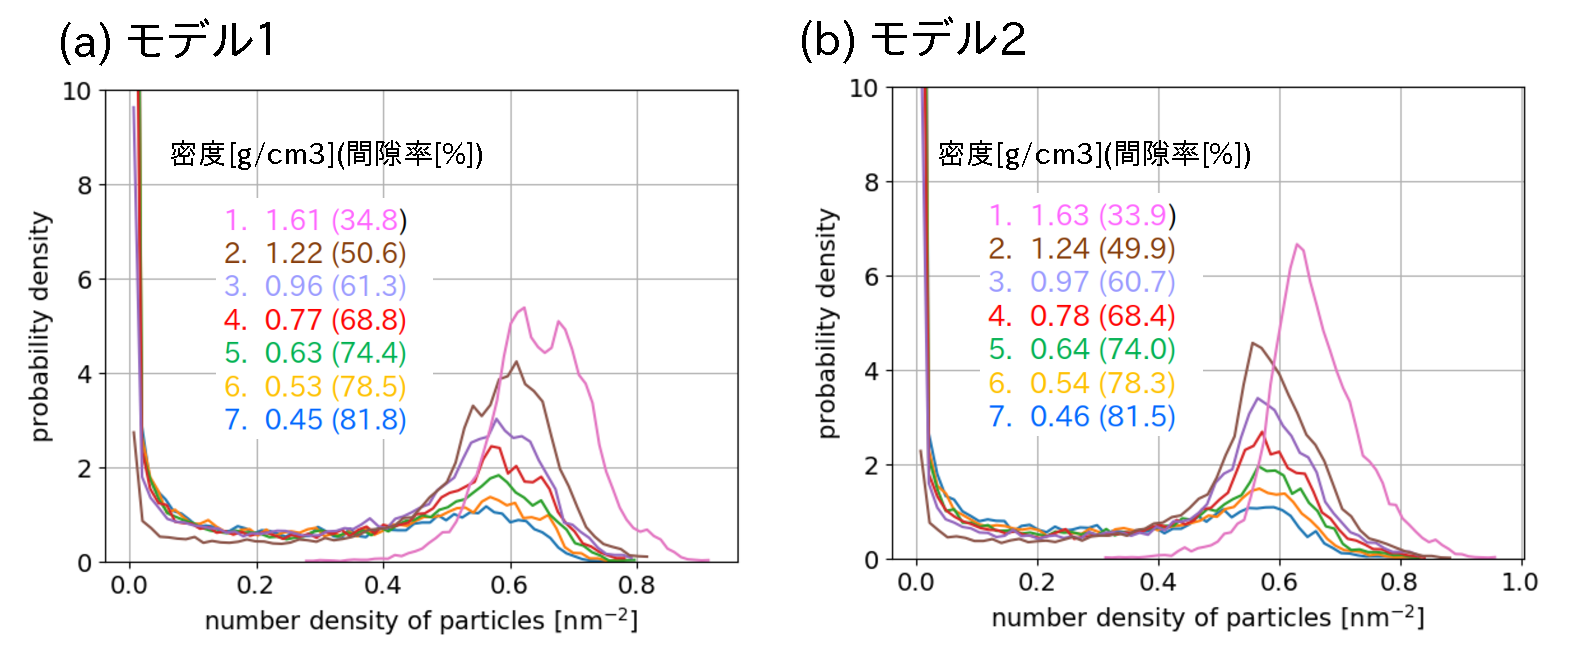
\includegraphics[width=1.0\linewidth]{Figs/fig8.eps} 
	\end{center}
	\caption{
		メソMDシミュレーションの結果から求めた数密度の確率確率密度分布.
	} 
	\label{fig:fig8}
\end{figure}
%--------------------
\subsubsection{空間分布の推移}
圧縮凝集過程における粒子数密度の推移を,図\ref{fig:fig10}と図\ref{fig:fig11}に示す.
これらは,粒子数密度の空間分布を,6つの時刻におけるスナップショットとして
示したものである.これらの図において,数密度が小さな領域は青で,大きな部分は赤で
示されている.ごく初期の段階から,0.8程度の数密度を持つ箇所が現れており,ここでも
粘土分子は早々に積層構造を作ることを示している.また,圧縮の途中段階で,積層構造が
あまり大きく発達しないことも分かる.なお,モデル1と2に対する結果において,
例えば図\ref{fig:fig11}の(a)と(d)を比較すると,モデル2の方がやや大きな空洞が
残されているように見えるが,その他の点で,2つのモデルで明確な違いは認められない.
ここに示されるように,粘土層間の微細な間隙(ナノ間隙)と層外の比較的大きな
間隙(メソ間隙)の分布を容易に定量化できる.スケールの異なる間隙では,
物質輸送挙動が異なることから,マクロスケールでの物質輸送解析を行う際,
空隙のサイズと連結性のモデルを与える必要がある.こで示した密度分布に基づく
間隙の区分は,そのようなモデル化作業において今後有用になると考えられる.
%--------------------
\begin{figure}[h]
	\begin{center}
	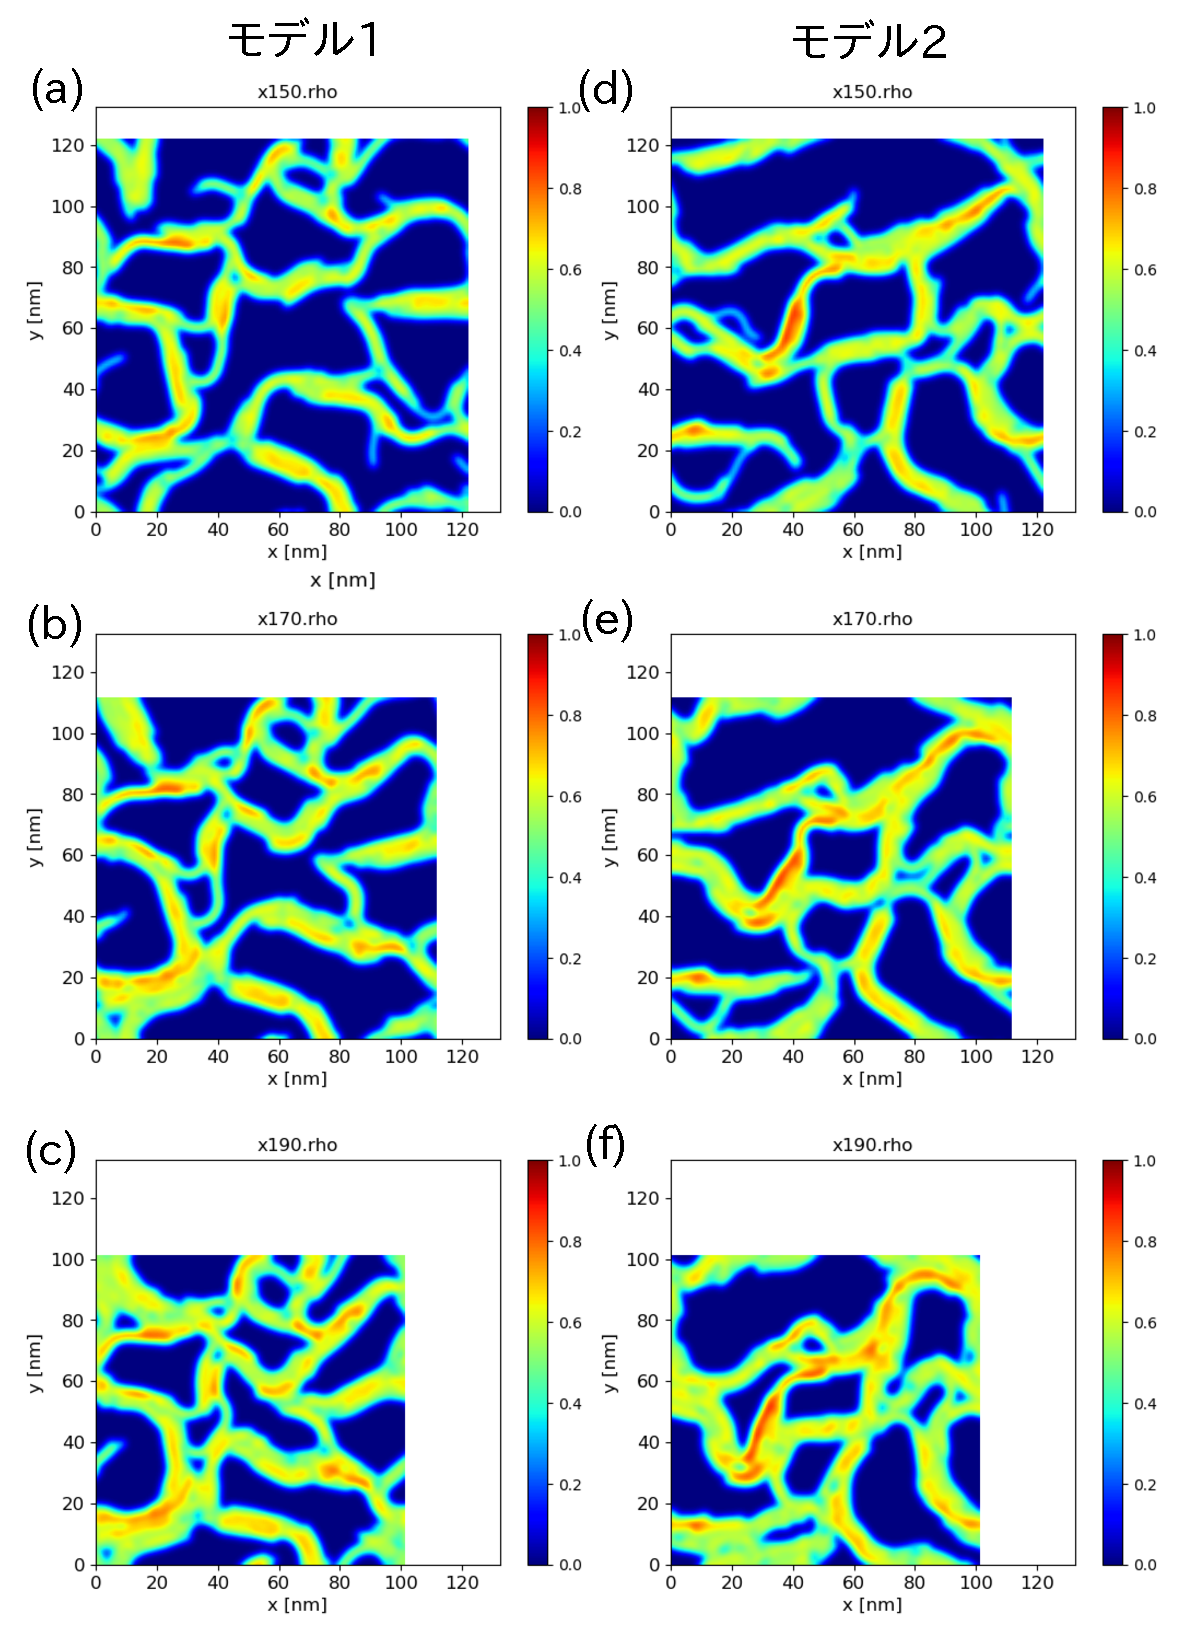
\includegraphics[width=1.0\linewidth]{Figs/fig10.eps} 
	\end{center}
	\caption{
		粒子数密度の空間分布(圧縮凝集過程の途中段階での状況を示すスナップショット).
	} 
	\label{fig:fig10}
\end{figure}
%--------------------
%--------------------
\begin{figure}[h]
	\begin{center}
	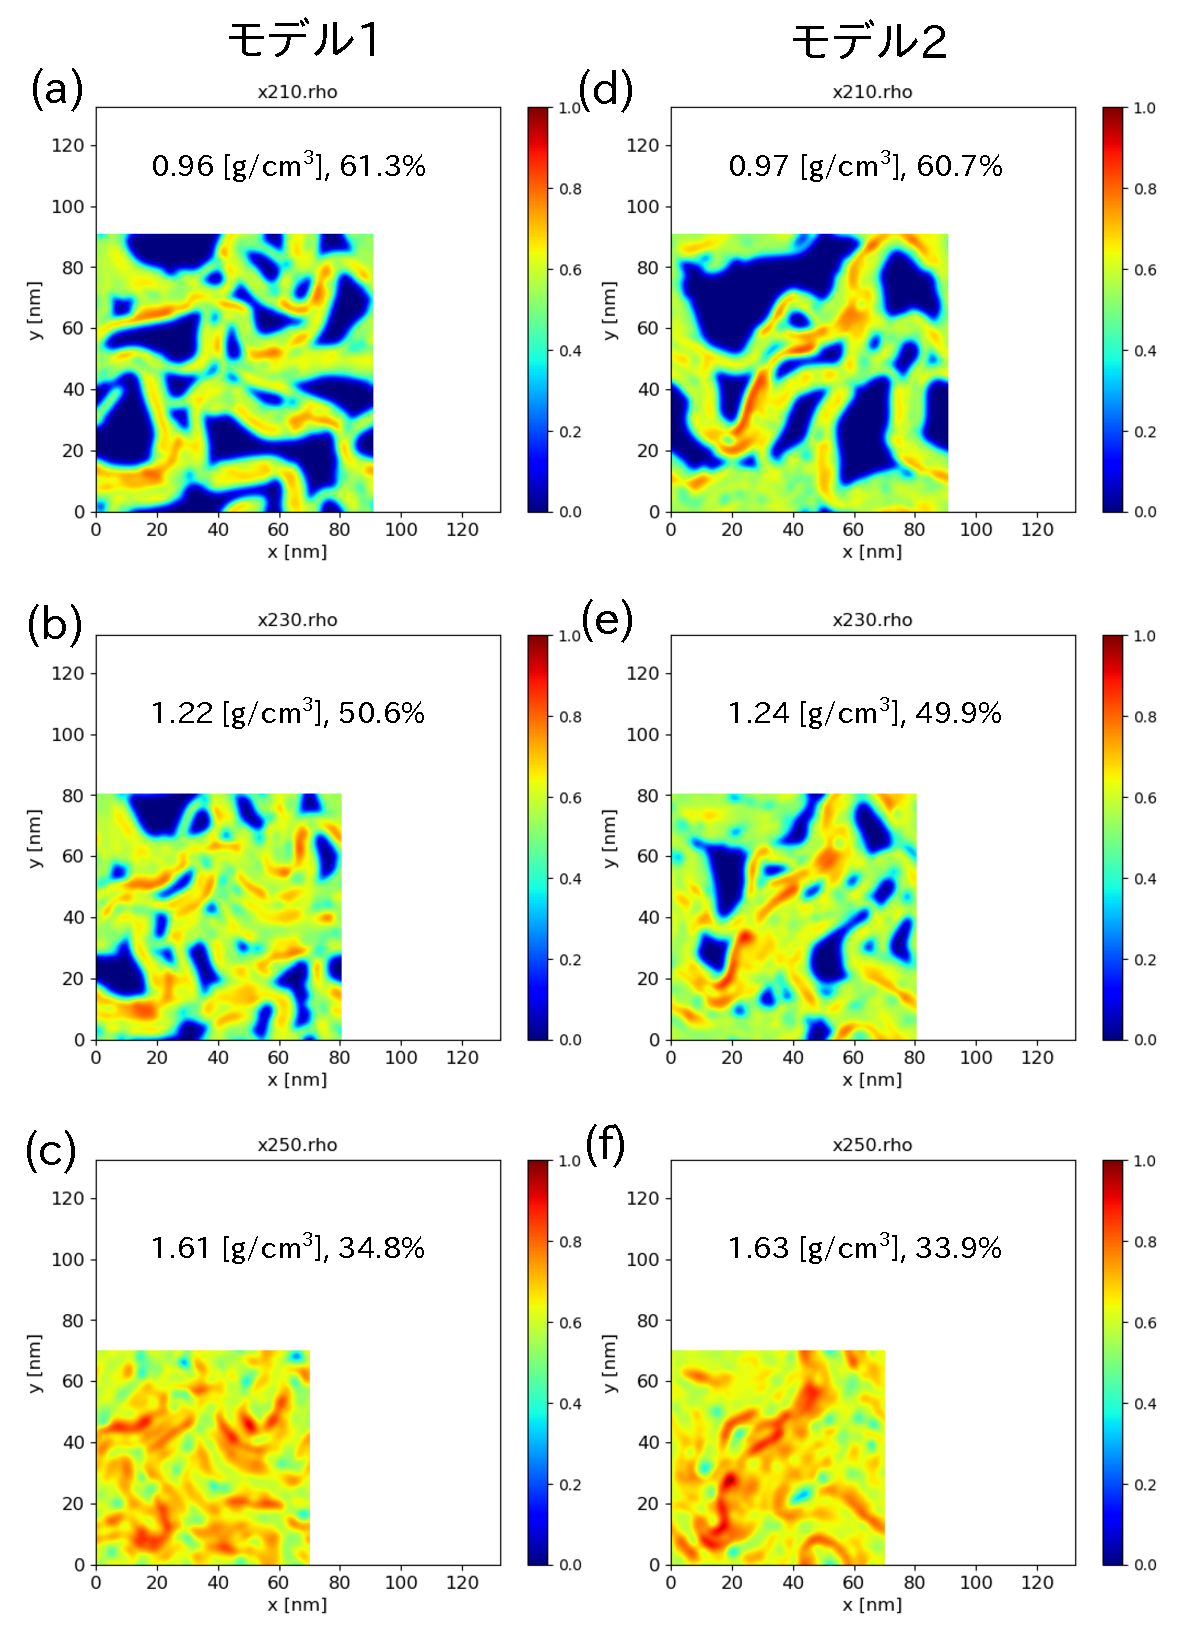
\includegraphics[width=1.0\linewidth]{Figs/fig11.eps} 
	\end{center}
	\caption{
		粒子数密度の空間分布(圧縮凝集過程の最終段階の状況を示すスナップショット).
	} 
	\label{fig:fig11}
\end{figure}
%--------------------
\subsection{粒子の配向性}
最後に,粗視化粒子の配向性について調べた結果を図\ref{fig:fig9}に示す.
このグラフは,ユニットセル中の全粗視化粒子の方向を調べ,粒子方向$\alpha$[deg]の
確率密度分布を求めた結果である.2つのモデルそれぞれ,7つの異なる乾燥密度における
結果を示していることは,これまでのグラフと同様である.
モデル1と2に対する結果を比較すると,モデル1の方がやや強く配向
している様子が示されている.モデル1はおよそ$\alpha=$100度の方向に配向
しており,その傾向が圧縮の進行中も持続している.このことは,積層構造を形成した
粘土分子群は,方向を変化させにくいことを示唆している.
さらに,そのような方向を変化させることに対する抵抗は,モデル1がモデル2に比べて強い
ことも示唆されている.こういった挙動は,拡散係数等の物性値に異方性に反映されると
予想されるため,明確な配向性が結果的に生じない場合においても,
組織構造解析の一貫として実施する価値があると思われる.
%--------------------
\begin{figure}[h]
	\begin{center}
	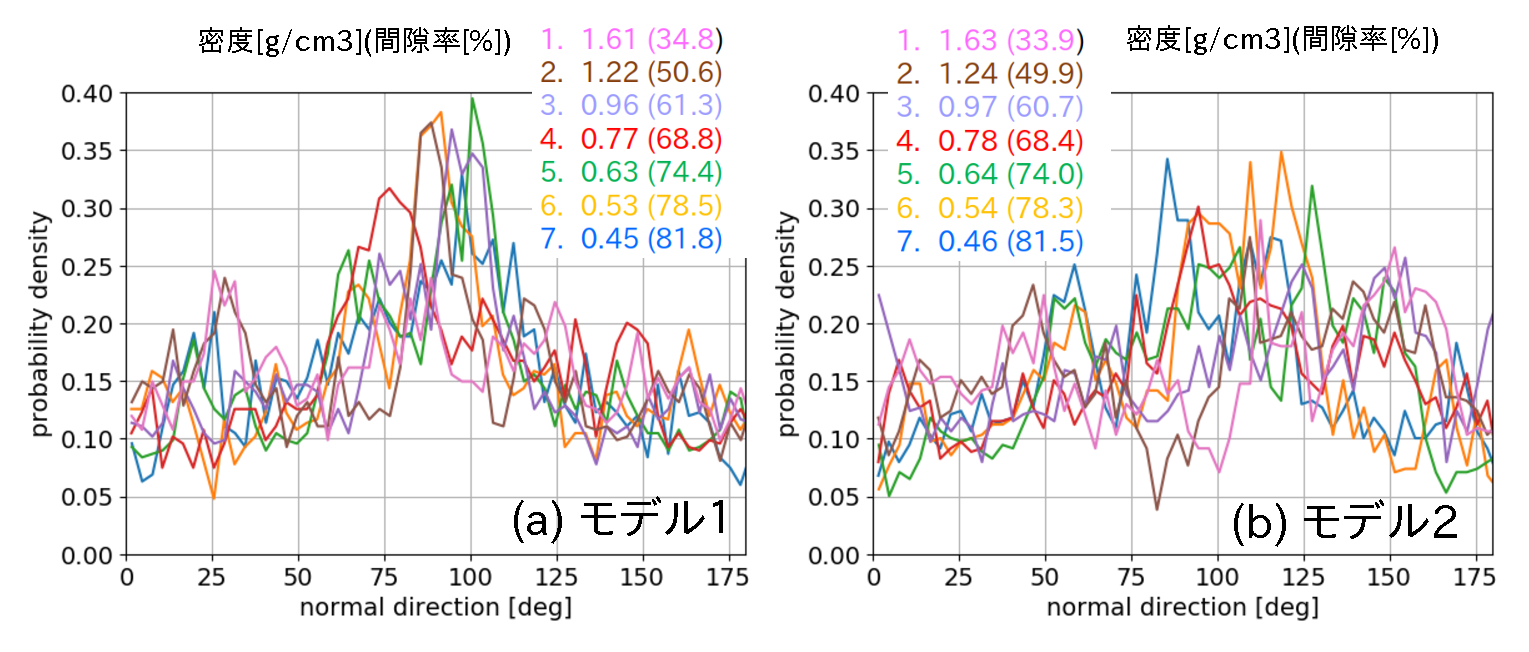
\includegraphics[width=1.0\linewidth]{Figs/fig9.eps} 
	\end{center}
	\caption{
		メソMDシミュレーションの結果から求めた粒子方向の確率密度分布.
	} 
	\label{fig:fig9}
\end{figure}
%--------------------
